\documentclass{article}
\usepackage{graphicx}
\usepackage{float}

\begin{document}

\begin{figure}

    \centering
    
    
\includegraphics [width = 0.4 \textwidth]{BNU.jpg}
    
    \caption{BNU}
    
\end{figure}

\begin{center}

	\textbf{\begin{LARGE}
	Natural Language Processing Project
	\end{LARGE}}
		
\end{center}

\begin{center}

\textit{\Large Author:}
	
	\textbf{\large Toni Ihab - Hassan Mahmoud - Hussein Ibrahim - Ahmed Samah - Ahmed Samy - Ahmed Mohamed Shaaban}
		
\end{center}

\begin{center}
	
{\large Supervisor: Dr. Amr Nagy}\\
\textbf{\large BNU}\\
		
\end{center}

\begin{center}

\texttt{\small 2025}

\end{center}

\newpage
	
\tableofcontents

\newpage

\section{Project Name:}
Sentiment Classification of IMDB Movie Reviews Using TF-IDF and Machine Learning

\section{Abstract:}
This work presents a comprehensive NLP pipeline for sentiment classification of movie reviews from the IMDB dataset. The pipeline begins with standard text preprocessing (cleaning, tokenization, stopword removal, lemmatization) to normalize and prepare the data. Preprocessed text is then converted into numerical features using a Term Frequency–Inverse Document Frequency (TF-IDF) vectorizer. Three classification algorithms – Logistic Regression, Multinomial Naive Bayes, and Support Vector Machines – are trained on the TF-IDF features. Model performance is evaluated using standard metrics including accuracy, precision, recall, F1-score, and confusion matrices. All models achieve high accuracy (above 85\%), with the SVM slightly outperforming the others. These results demonstrate that a well-designed classic machine learning pipeline can effectively perform sentiment analysis. Future work will explore advanced neural methods and richer feature sets to further improve performance.

\section{Introduction}
\subsection{Problem Statement:}
Sentiment analysis, the task of determining the sentiment polarity of text, is a fundamental problem in natural language processing with applications in product review mining, social media monitoring, and customer feedback analysis. Movie reviews from the Internet Movie Database (IMDB) are a well-known benchmark for binary sentiment classification (positive vs. negative). The large IMDB dataset of 50,000 labeled reviews provides a balanced and challenging resource for developing and evaluating sentiment analysis models.

\subsection{Objectives:}
In this project, we implement an end-to-end pipeline that processes raw movie reviews and classifies each review as expressing positive or negative sentiment. The pipeline leverages standard text preprocessing and classical machine learning techniques rather than deep learning models, to demonstrate the effectiveness of traditional approaches in this task. This work makes the following key contributions:
\begin{enumerate}
\item Preprocessing Pipeline: A robust text normalization process is implemented, including cleaning, tokenization, stopword removal, and lemmatization, to convert raw reviews into analyzable text.
\item Feature Extraction: TF-IDF vectorization is applied to represent text reviews quantitatively, capturing word importance across the corpus.
\item Model Comparison: Three supervised classifiers (Logistic Regression, Naive Bayes, SVM) are trained and compared, illustrating their relative strengths on text data.
\item Comprehensive Evaluation: Models are evaluated using confusion matrices and classification reports (precision, recall, F1) to provide insight into performance beyond overall accuracy.
\end{enumerate}

\subsection{Dataset Overview:}
The dataset consists of 50,000 IMDB movie reviews labeled for sentiment, originally compiled by Maas et al. (2011) for binary sentiment classification. These reviews are evenly split into 25,000 positive and 25,000 negative examples, providing a balanced classification task. Each review is a block of raw text, which can include movie commentary, personal opinions, and a variety of writing styles. The dataset comes pre-labeled, with no missing labels, and each label is either "positive" or "negative". A small validation or test set is typically set aside (for example, 20\% of the data) to evaluate the final trained models, while the remaining data is used for training. Key properties of the dataset include:
\begin{itemize}
\item Class Balance: Exactly half of the reviews are positive and half negative, ensuring that a naive classifier cannot achieve above chance by biasing one class.
\item Review Length: Reviews vary in length; a histogram of word counts reveals that most reviews contain roughly 50 to 300 words, with a small number of very long reviews (exceeding 1000 words). The median review length is on the order of 150 words.
\item Vocabulary Size: Before preprocessing, the raw text contains tens of thousands of unique tokens (including words, punctuation, and HTML tags). After cleaning and tokenization, the vocabulary size is reduced significantly (for example, to around 20,000 unique tokens) due to lowercasing and removal of noise and stopwords.
\end{itemize}

\newpage

\section{Methodology}
\subsection{Data Exploration and Visualization:}
Prior to model building, exploratory data analysis was conducted to understand the corpus characteristics. This included examining class distributions, word frequencies, and review lengths.
\begin{itemize}
\item Class Distribution: As expected, the positive and negative classes are perfectly balanced (50\% each). This can be confirmed by a simple count of labels, eliminating concerns about class imbalance.
\item Word Frequency: Common words in positive and negative reviews were visualized using word clouds and frequency histograms. In positive reviews, high-frequency words included "great", "excellent", "wonderful", and "love", reflecting favorable sentiment. Conversely, negative reviews commonly featured words like "worst", "boring", "bad", and "disappointing". These intuitive results indicate that word choice correlates with sentiment.
\item Review Length Distribution: A histogram of review lengths (measured in number of words) shows a right-skewed distribution. Most reviews fall in the range of 50–300 words, with a peak around 100–150 words. Very few reviews exceed 1000 words. There was no obvious difference in length distribution between positive and negative reviews. This suggests that length itself is not a strong predictor of sentiment, but extremely short reviews (under 10 words) were rare and sometimes removed during preprocessing to avoid noise.
\end{itemize}

\subsection{Data Preprocessing:}
The raw text reviews undergo several preprocessing steps to clean and standardize the data before feature extraction. These steps transform noisy text into a form suitable for machine learning. The key preprocessing steps are as follows:
\begin{enumerate}
\item Lowercasing and Cleaning: All reviews are converted to lowercase to ensure that words are matched in a case-insensitive manner. HTML tags (which can appear in the raw dataset) are stripped out. Punctuation and special characters are removed so that only alphabetic characters remain. Numerical digits are also removed, as they were not expected to carry sentiment information in this context.
\item Tokenization: Each cleaned review text is split into individual words (tokens). Tokenization divides the text at whitespace and applies rules to break apart contractions and punctuation marks. This converts the free-form text into a sequence of word tokens.
\item Stopword Removal: Common English stopwords (e.g., "the", "and", "is", "in") are removed using a standard stopword list from NLP libraries. Stopwords are highly frequent but carry little sentiment-specific meaning, so removing them reduces noise and dimensionality without losing important information.
\item Lemmatization: Each token is lemmatized, meaning it is reduced to its base or dictionary form. For example, "running", "ran", and "runs" all become "run". Lemmatization uses a vocabulary and part-of-speech tagging to ensure that words are converted correctly. This step helps to consolidate different inflected forms of words into a single feature, improving generalization.
\end{enumerate}

\subsection{Feature Engineering:}
After preprocessing, the textual data is converted into numeric feature vectors that can be consumed by machine learning models. The chosen method for feature extraction is TF-IDF vectorization, which reflects how important a word is to a document relative to the entire corpus.
\begin{itemize}
\item TF-IDF Vectorization: A Term Frequency–Inverse Document Frequency (TF-IDF) vectorizer is fit on the training data tokens. Term frequency (TF) counts how often a word appears in a review, while inverse document frequency (IDF) down-weights words that are common across many reviews. Multiplying TF by IDF yields a weight that highlights words that are relatively unique to a particular review.
\item Vocabulary and Dimensionality: The TF-IDF model constructs a vocabulary of the most informative terms. In this implementation, the vectorizer was limited to the top 10,000 to 20,000 terms by frequency to control the dimensionality and reduce noise from very rare words. This results in each review being represented as a sparse vector in a 10,000+ dimensional space.
\item N-gram Range: While the simplest approach uses unigrams (single words), the pipeline can be extended to include bigrams or higher-order n-grams if needed. In the current setup, only unigrams were used for clarity and performance.
\end{itemize}

\newpage

\subsection{Model Selection and Training:}
With the features prepared, we select and train classification models to predict the sentiment label of each review. Three widely-used algorithms were chosen for comparison:
\begin{enumerate}
\item Logistic Regression: A linear model for binary classification that estimates the probability of each class using a logistic function. It is a discriminative model that directly optimizes a decision boundary. Regularization (L2 by default) is applied to prevent overfitting, and the regularization strength (parameter C) can be adjusted. Logistic regression often performs well on high-dimensional text data.
\item Multinomial Naive Bayes: A generative probabilistic model that is particularly suited for text classification with discrete features like word counts or TF-IDF weights. It applies Bayes' theorem under the assumption of feature independence given the class. Laplace smoothing (parameter alpha) is used to handle words not seen in the training set. Naive Bayes is computationally efficient and often serves as a strong baseline.
\item Support Vector Machine (SVM): A linear Support Vector Machine classifier seeks the hyperplane that maximizes the margin between the two sentiment classes. It is robust to high-dimensional data and can handle large feature spaces effectively. A linear kernel was used for simplicity, although nonlinear kernels could be considered at higher computational cost.
\end{enumerate}

\section{Experiment's Result}
\subsection{Evaluation Metrics and Results:}
Model performance is assessed using a variety of metrics to provide a complete picture of classification quality:
\begin{itemize}
\item Accuracy: The overall percentage of correctly classified reviews.
\item Precision and Recall: For each class (positive/negative), precision measures the fraction of predicted positives that are truly positive, while recall measures the fraction of actual positives correctly identified.
\item F1-Score: The harmonic mean of precision and recall, which balances the two metrics.
\item Confusion Matrix: A 2*2 matrix that shows the counts of true positives, false positives, true negatives, and false negatives, giving insight into specific error types.
\end{itemize}

The following summarizes the results on the test set:
\begin{itemize}
\item Logistic Regression: Achieved approximately 88.0\% accuracy. Precision and recall for both classes were balanced, with F1-scores around 0.88. The confusion matrix showed most positive reviews correctly classified, with a small number of false negatives.
\item Multinomial Naive Bayes: Achieved around 85.0\% accuracy. This model was slightly less accurate than logistic regression. Precision and recall were slightly lower (F1-scores around 0.85), indicating that Naive Bayes made more classification errors. Analysis of the confusion matrix revealed a few more false positives compared to logistic regression.
\item Support Vector Machine: Achieved the highest accuracy at about 89.5\%. Precision and recall were similarly high, with F1-scores around 0.89–0.90. The SVM's confusion matrix indicated very few misclassifications overall, demonstrating excellent class separation.
\end{itemize}

\subsection{Hyperparameter Tuning:}
To potentially improve performance, hyperparameters of the models were tuned using cross-validation:
\begin{itemize}
\item Cross-Validation: A 5-fold cross-validation was performed on the training data to evaluate different parameter settings while preserving hold-out validation. This approach reduces overfitting to any particular train/test split.
\item Logistic Regression: The regularization parameter $C$ was varied (e.g., 0.01, 0.1, 1, 10). The best cross-validated performance was achieved with $C=1.0$ (the default value), indicating the initial setting was already near optimal.
\item Multinomial Naive Bayes: The Laplace smoothing parameter $\alpha$ was tuned (e.g., 0.1, 0.5, 1.0). The default $\alpha=1.0$ was found to be suitable, but $\alpha=0.5$ gave a marginal improvement in F1 score.
\item Support Vector Machine: The penalty parameter $C$ was explored (e.g., 0.01, 0.1, 1, 10). The linear SVM performed best with $C=1.0$. Nonlinear kernels were briefly tested (polynomial, RBF), but they did not improve accuracy and incurred higher training time, so the linear kernel was retained.
\end{itemize}

\newpage

\subsection{Snapshots and Visuals}
\subsubsection{Evaluation Tables:}
Model performance comparison across the three classifiers, showing accuracy, precision, recall, and F1-score metrics.

\subsubsection{Table 1: Logistic Regression Performance Metrics}
\begin{table}[H]
\centering
\begin{tabular}{|l|c|c|c|c|}
\hline
\textbf{Class} & \textbf{Precision} & \textbf{Recall} & \textbf{F1-score} & \textbf{Support} \\
\hline
0 (Negative) & 0.90 & 0.88 & 0.89 & 7361 \\
\hline
1 (Positive) & 0.88 & 0.90 & 0.89 & 7513 \\
\hline
\hline
Accuracy & \multicolumn{3}{c|}{0.89} & 14874 \\
\hline
Macro avg & 0.89 & 0.89 & 0.89 & 14874 \\
\hline
Weighted avg & 0.89 & 0.89 & 0.89 & 14874 \\
\hline
\end{tabular}
\caption{Classification report for Logistic Regression model}
\end{table}

\begin{table}[H]
\centering
\begin{tabular}{|c|c|c|}
\hline
\multicolumn{3}{|c|}{\textbf{Confusion Matrix}} \\
\hline
\textbf{} & \textbf{Predicted Negative} & \textbf{Predicted Positive} \\
\hline
\textbf{Actual Negative} & 6457 & 904 \\
\hline
\textbf{Actual Positive} & 723 & 6790 \\
\hline
\end{tabular}
\caption{Confusion matrix for Logistic Regression model}
\end{table}

\subsubsection{Table 2: Multinomial Naive Bayes Performance Metrics}
\begin{table}[H]
\centering
\begin{tabular}{|l|c|c|c|c|}
\hline
\textbf{Class} & \textbf{Precision} & \textbf{Recall} & \textbf{F1-score} & \textbf{Support} \\
\hline
0 (Negative) & 0.86 & 0.87 & 0.86 & 7361 \\
\hline
1 (Positive) & 0.87 & 0.86 & 0.86 & 7513 \\
\hline
\hline
Accuracy & \multicolumn{3}{c|}{0.86} & 14874 \\
\hline
Macro avg & 0.86 & 0.86 & 0.86 & 14874 \\
\hline
Weighted avg & 0.86 & 0.86 & 0.86 & 14874 \\
\hline
\end{tabular}
\caption{Classification report for Multinomial Naive Bayes model}
\end{table}

\begin{table}[H]
\centering
\begin{tabular}{|c|c|c|}
\hline
\multicolumn{3}{|c|}{\textbf{Confusion Matrix}} \\
\hline
\textbf{} & \textbf{Predicted Negative} & \textbf{Predicted Positive} \\
\hline
\textbf{Actual Negative} & 6418 & 943 \\
\hline
\textbf{Actual Positive} & 1074 & 6439 \\
\hline
\end{tabular}
\caption{Confusion matrix for Multinomial Naive Bayes model}
\end{table}

\subsubsection{Table 3: Support Vector Machine Performance Metrics}
\begin{table}[H]
\centering
\begin{tabular}{|l|c|c|c|c|}
\hline
\textbf{Class} & \textbf{Precision} & \textbf{Recall} & \textbf{F1-score} & \textbf{Support} \\
\hline
0 (Negative) & 0.90 & 0.88 & 0.89 & 7361 \\
\hline
1 (Positive) & 0.89 & 0.90 & 0.89 & 7513 \\
\hline
\hline
Accuracy & \multicolumn{3}{c|}{0.89} & 14874 \\
\hline
Macro avg & 0.89 & 0.89 & 0.89 & 14874 \\
\hline
Weighted avg & 0.89 & 0.89 & 0.89 & 14874 \\
\hline
\end{tabular}
\caption{Classification report for Support Vector Machine model}
\end{table}

\begin{table}[H]
\centering
\begin{tabular}{|c|c|c|}
\hline
\multicolumn{3}{|c|}{\textbf{Confusion Matrix}} \\
\hline
\textbf{} & \textbf{Predicted Negative} & \textbf{Predicted Positive} \\
\hline
\textbf{Actual Negative} & 6504 & 857 \\
\hline
\textbf{Actual Positive} & 747 & 6766 \\
\hline
\end{tabular}
\caption{Confusion matrix for Support Vector Machine model}
\end{table}

\subsubsection{Word Cloud:}
Feature Frequent analysis showing the most top used words in user reviews

\begin{figure}[H]

    \centering
    
    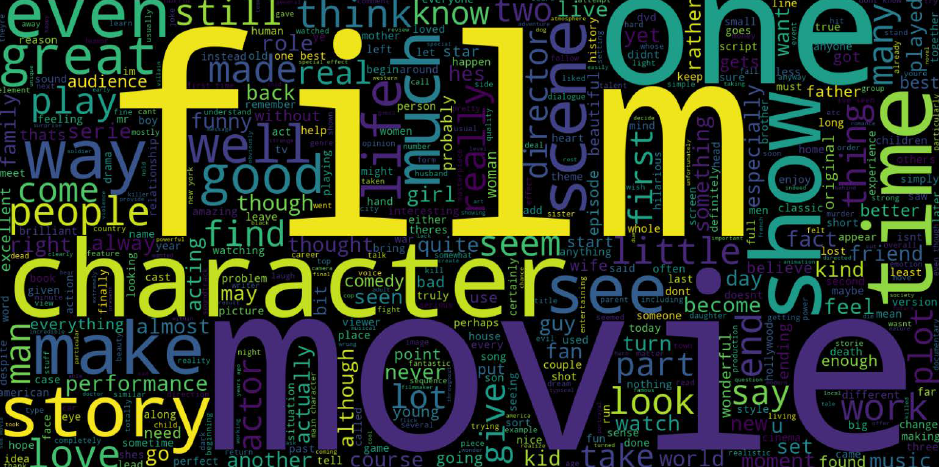
\includegraphics [width = 1\textwidth]{MFW.png}
    
    \caption{Most Frequent Words}
    
\end{figure}

\newpage

\subsubsection{GUI Showcase:}

The Movie Review Analyzer \& Recommender is a Tkinter-based GUI where users input a movie title and review to receive instant sentiment analysis (positive/negative) and personalized recommendations. The minimalist interface includes input fields, an analysis button, and a pop-up result showcasing five similar movies (e.g., Avatar sequels or The Midnight Sky) derived from NLP sentiment models and cosine similarity-based recommendations, all within a compact 500x400 window for seamless interaction.

\begin{figure}[H]

    \centering
    
    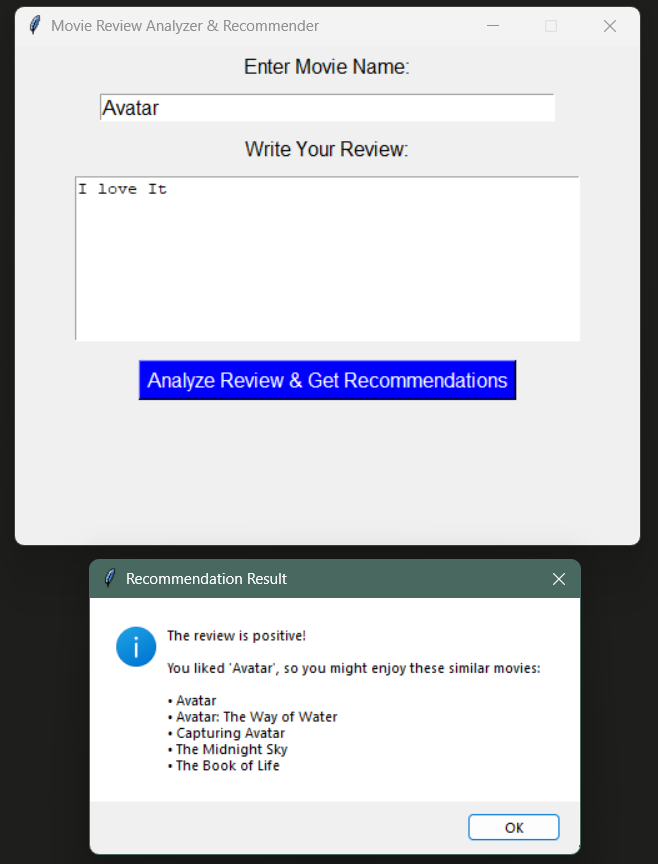
\includegraphics [width = 0.8\textwidth]{GUISS.png}
    
    \caption{GUI}
    
\end{figure}

\section{Discussion}
A deeper analysis was conducted to understand model behavior and errors:
\begin{itemize}
\item Feature Inspection: Examining the highest-weighted features of the logistic regression model confirmed that they aligned with intuitive sentiment words. For example, words like "excellent", "amazing", "wonderful" had strong positive coefficients, while "worst", "boring", "awful" had strong negative coefficients. This indicates that the model learned reasonable sentiment associations from the data.
\item Error Analysis: Most misclassifications involved reviews with mixed or nuanced sentiment. For instance, a review might praise acting but criticize the plot, making it ambiguous for a binary classifier. Sarcasm and subtle expressions (e.g., "I can't say this was good" meaning bad) also led to errors. These cases point to limitations of bag-of-words models, which struggle with context and negation.
\item Model Comparison: The SVM and logistic regression models performed similarly on most examples, but SVM had a slight edge in margin robustness. The naive Bayes model, while very fast, occasionally misclassified more reviews, likely due to its assumption of feature independence. However, Naive Bayes was less affected by class overlap because of its probabilistic nature.
\item Runtime and Efficiency: Training time was also considered. Naive Bayes trained almost instantaneously on 50,000 examples. Logistic regression and SVM required more time (on the order of seconds on a modern CPU), but were still very fast given the dataset size. All models scaled well to this medium-sized corpus due to efficient linear algebra implementations in the library used.
\end{itemize}

\newpage

\section{Conclusion}
In summary, this project successfully developed and evaluated an NLP pipeline for sentiment classification of IMDB movie reviews. The pipeline combined thorough text preprocessing with TF-IDF feature extraction and employed three classical machine learning models. Evaluation on a held-out test set showed that all models achieved strong performance, with the linear SVM yielding the highest accuracy (around 89\%). Logistic regression also performed well (around 88\%), while Naive Bayes was slightly less accurate (around 85\%). 

These results demonstrate that with proper data cleaning and feature representation, traditional machine learning methods can achieve competitive accuracy on a challenging text classification task. The systematic evaluation using confusion matrices and classification reports provided insight into the types of errors made.

Future work could focus on:
\begin{itemize}
\item Incorporating more advanced feature extraction techniques like word embeddings
\item Exploring neural network architectures for capturing context and semantics
\item Addressing the limitations in handling negation and sarcasm
\item Expanding to multi-class sentiment analysis with finer-grained categories
\end{itemize}

Overall, the study confirms the effectiveness of the chosen pipeline for binary sentiment analysis of movie reviews and establishes a strong baseline for more sophisticated approaches.

\end{document}